\documentclass{article}
\usepackage{tikz}
\usepackage{amsmath}

\begin{document}

\section*{Overview of How to Construct a New Generation}

The process of constructing a new generation involves the following steps:
1. Order the genes from best to worst in the current generation.
2. Discard the worst genes, which correspond to the red part of the diagram.
3. Copy the best genes directly into the new generation, corresponding to the green part.
4. Generate the remaining genes in the new generation by performing crossovers between genes from the green part and gray part of the previous generation.

\begin{center}
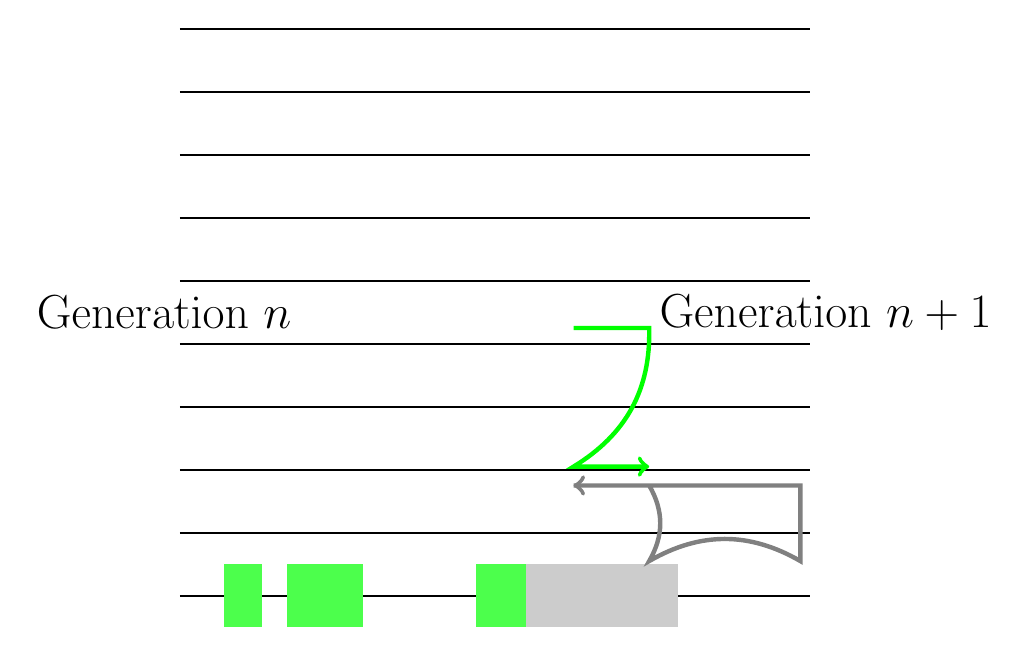
\begin{tikzpicture}[scale=0.8]
    % Draw vertical lines for the generations
    \foreach \y in {1,...,10} {
        \draw [thick] (-0.5,\y) -- ++(10,0);
    }
    
    % Draw the red gene in generation n
    \fill [red!70] (0.2, 0.5) rectangle ++(0.6, 1);
    
    % Draw the green genes in both generations
    \foreach \x in {0.2, 1.2, 1.8, 4.2, 4.8, 5.4} {
        \fill [green!70] (\x, 0.5) rectangle ++(0.6, 1);
    }
    
    % Draw the gray genes in generation n
    \foreach \x in {5, 5.6, 6.2, 6.8} {
        \fill [gray!40] (\x, 0.5) rectangle ++(0.6, 1);
    }
    
    % Draw the green arrow to indicate copying genes
    \draw[ultra thick, ->, green] (5.75, 5.25) -- ++(1.2, 0) to[bend left] ++(-1.2, -2.2) -- ++(1.2, 0);
    
    % Draw the gray arrow to indicate crossover
    \draw[ultra thick, ->, gray] (5.75, 2.75) -- ++(1.2, 0) -- ++(2.4, 0) -- ++(0, -1.2) to[bend right] ++(-2.4, 0) to[bend right] ++(0, 1.2) -- ++(-1.2, 0);
    
    % Label the generations
    \node at (-0.75, 5.5) {\LARGE Generation $n$};
    \node at (9.75, 5.5) {\LARGE Generation $n+1$};
\end{tikzpicture}
\end{center}

\end{document}